\subsection{Analoges Theremin}\label{subsec:Theremin_analog}
Das klassische Theremin besitzt zwei Antennen. Der Spieler kann über die senkrecht angebrachte Antenne  die  Tonhöhe beeinflussen. Mit der waagrechten Antenne regelt der Spieler die Lautstärke. Eine typische Eigenschaft des Theremins ist, dass der Ton des Theremins in einem weiten Frequenzbereich kontinuierlich veränderbar ist. Das Theremin kann daher alle Frequenzen in einem Bereich spielen, im Gegensatz zu den meisten anderen Instrumenten.

Der Spieler spielt das Theremin durch verstimmen der Oszillatoren über die Antennen.
Die Hand des Spielers verändert über die jeweilige Antenne die Schwingfrequenz des Tonhöhen- und Lautstärkenoszillators. Dabei wird der kapazitive Anteil des LC-Schwingkreises beeinflusst, was eine Änderung der Schwingfrequenz zur Folge hat. 
Die Frequenz dieser Oszillatoren ist jedoch weit über dem hörbaren Bereich (zwischen \SI{100}{kHz} bis \SI{1}{MHz}). Mit Hilfe eines Mischers und einem Referenzoszillator wird die Frequenzdifferenz des Tonhöhenoszillators hörbar gemacht und danach verstärkt\cite{Franzis}. Der Lautstärkepegel ergibt sich durch die Verwendung eines Bandpassfilters und eines nachfolgenden Hüllkurvendetektors. Die Abbildung \ref{img:Blockschaltbild_analog} gibt einen Überblick über die Schaltungskomponenten eines Theremins. Die einzelnen Schaltungsteile sind im folgenden Teil genauer erklärt.

\begin{figure}[h]
	\centering
	\includegraphics[width=0.8\textwidth]{Blockschaltbild_analog.pdf}
	\caption{Blockschaltbild eines analogen Theremins}
	\label{img:Blockschaltbild_analog}
\end{figure}

\paragraph{Tonhöhenoszillator und Tonhöhenantenne}\mbox{}\\

Die Tonhöhenantenne ist ein Metallrohr, welches mit dem Tonhöhenoszillator verbunden ist.
Der Spieler kann über die Distanz seiner Hand zur Antenne die Frequenz des Tonhöhenoszillator verändern. Die über die Antenne zu erreichende Kapazitätsänderung ist sehr gering. Diese liegt im Picofarad Bereich \cite{physik_theremin}. Die Grundfrequenz des Tonhöhenoszillators muss weit über dem hörbaren Bereich liegen, damit eine genügend grosse Frequenzänderung entsteht.

\paragraph{Lautstärkenoszillator und Lautstärkenantenne}\mbox{}\\ 

Die Lautstärkenantenne ist wie die Tonhöhenantenne ein Metallrohr, welches mit dem Lautstärkenoszillator verbunden ist. Die durch den Spieler beeinflusste Frequenzänderung wandelt ein Hüllkurvendetektor in eine Spannung um. Diese Spannung dient dem Verstärker als Steuergrösse, um das Audio Signal zu verstärken. \cite{Franzis}. 

\paragraph{Mischer und Referenzoszillator}\mbox{}\\ 
\\Die erzeugte Frequenz der Tonhöhenantenne liegt weit über dem vom Menschen hörbaren Bereich. Der Mischer multipliziert die Signale des Referenzoszillators und des Tonhöhenoszillators wie in Formel \ref{equ:mischer}. $A_1\sin(\omega_1t)$ entspricht dem Signal des Referenzoszillators und $A_2\sin(\omega_2t)$ dem Signal des Tonhöhenoszillators.

\begin{equation}
V_{out} = A_{1}A_{2} \sin(\omega_{1}t)   \sin(\omega_{2}t) 
\label{equ:mischer}
\end{equation}

$V_{out}$ kann durch Additionstheoreme umgeformt werden. Dabei erhält man folgenden Ausdruck:

\begin{equation}
V_{out} = A/2[\cos((\omega_{1}-\omega_{2})t)  - \cos((\omega_{1}+\omega_{2})t) ]
\label{equ:mischer_trigo}
\end{equation}

Das Ausgangssignal $V_{out}$ hat zwei Frequenzkomponenten. Zum einen die Differenz der beiden Frequenzen, zum anderen die Summe der Frequenzen. Dabei ist bei dem Theremin nur die Differenz der Frequenzen von Interesse \cite{physik_theremin}.

Eine Kalibration des Theremins ist vor jedem Gebrauch nötig. Es könnte beispielsweise sein, dass die Differenz der Frequenz ausserhalb des hörbaren Bereiches liegt. Dazu stellt der Spieler beim klassischen Theremin mit Hilfe eines Trimmkondensators am Referenzoszillator die Differenzfrequenz auf \SI{0}{Hz} ein.

\paragraph{Tiefpassfilter}\mbox{}\\ 
\\Das Tiefpassfilter filtert die hochfrequente Komponente aus Formel \ref{equ:mischer_trigo} weg. Übrig bleibt die Differenz der Oszillatorfrequenzen. Dies ist der interessante Anteil des Mischprozesses, da er im hörbaren Bereich liegt.
\begin{equation}
V_{out} = A/2cos((\omega_{1}-\omega_{2})t) 
\label{equ:mischer_gefilt}
\end{equation}

\paragraph{Verstärker und  Lautsprecher}\mbox{}\\ 
\\Der Verstärker verstärkt das Ausgangssignal des Tiefpassfilters abhängig von der Spannung, welche vom Hüllkurvendetektor stammt.
